
=========================================================

ہم متعدد تعداد کے نقطہ منبع پر مبنی مختلف اقسام کے اینٹینا دیکھ چکے ہیں۔اگر متعدد نقطہ منبع کی قطار میں منبع کے درمیان فاصلہ اتنا کم کر دیا جائے کہ یہ علیحدہ علیحدہ منبع کی جگہ ایک مسلسل چادر نظر آئے تو ایسی صورت میں مسلسل اینٹینا حاصل ہو گا۔شکل \حوالہ{شکل_اینٹینا_مسلسل_اینٹینا} میں ایسا ہی اینٹینا دکھایا گیا ہے جس میں تمام نقطہ منبع کو ہم قدم برقی رو مہیا کی گئی ہے۔اس اینٹینے کی کل لمبائی \عددیء{a} کے برابر ہے۔اینٹینا \عددیء{y} محدد پر ہے۔  

\begin{figure}
\centering
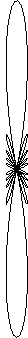
\includegraphics{emtAntennasAndRadiationContinuousAperture}
\caption{مسلسل اینٹینا}
\label{شکل_اینٹینا_مسلسل_اینٹینا}
\end{figure}

اینٹینا کے چھوٹے حصے \عددیء{\dif y} کا دور میدان \عددیء{\dif E}
\begin{align}
\dif E=\frac{A}{r_1} e^{j\omega (t -\frac{r_1}{c})} \dif y=\frac{A}{r_1} e^{j(\omega t -\beta r_1)} \dif y
\end{align}
لکھا جا سکتا ہے جہاں \عددیء{A} برقی رو پر منحصر مستقل ہے۔یوں مکمل اینٹینا کا میدان
\begin{align}
E=\int \limits_{-\frac{a}{2}}^{\frac{a}{2}} \frac{A}{r_1} e^{j(\omega t -\beta r_1)} \dif y
\end{align}
ہو گا۔شکل سے \عددیء{r_1=r-y\sin \theta} لکھا جا سکتا ہے۔یوں
\begin{align}
E=e^{j(\omega t -\beta r)}\int \limits_{-\frac{a}{2}}^{\frac{a}{2}} \frac{A}{r_1} e^{j \beta y\sin \theta} \dif y
\end{align}
حاصل ہوتا ہے۔اگر \عددیء{r_1 \gg a} ہو تب تکمل کے \عددیء{e^{j \beta y \sin \theta}} جزو کی قیمت \عددیء{y} تبدیل ہونے سے  اتنی تبدیل ہوتی ہے کہ اس تبدیلی کو نظر انداز نہیں کیا جا سکتا۔اس کے برعکس \عددیء{\tfrac{A}{r_1}} کی قیمت میں تبدیلی قابل نظر انداز ہے لہٰذا اس کو مستقل \عددیء{\tfrac{A}{r_1} \approx \tfrac{A}{r}} تصور کرتے ہوئے تکمل کے باہر لے جایا جا سکتا ہے۔یوں  
\begin{align}
E=\frac{A}{r}e^{j(\omega t -\beta r)}\int \limits_{-\frac{a}{2}}^{\frac{a}{2}} e^{j \beta y\sin \theta} \dif y
\end{align}
لکھا جا سکتا ہے۔تکمل لیتے ہوئے
\begin{gather}
\begin{aligned}\label{مساوات_اینٹینا_مسلسل}
E&=\frac{A}{r}e^{j(\omega t -\beta r)} \left[\frac{e^{j \beta\frac{a}{2} \sin \theta}}{j \beta\sin \theta} -\frac{e^{-j \beta\frac{a}{2} \sin \theta}}{j \beta\sin \theta} \right]\\
&=A' \frac{\sin \left(\frac{\beta a }{2} \sin \theta \right)}{\frac{\beta a }{2}\sin \theta}
\end{aligned}
\end{gather}
حاصل ہوتا ہے جہاں
\begin{align*}
\frac{a Ae^{j(\omega t -\beta r)}}{r}=A'
\end{align*}
لکھا گیا ہے۔

مساوات \حوالہ{مساوات_اینٹینا_مسلسل} زیادہ سے زیادہ میدان \عددیء{\theta=90^{\circ}} پر \عددیء{A'} دیتا ہے۔یوں مساوات \حوالہ{مساوات_اینٹینا_مسلسل} کو \عددیء{A'} سے تقسیم کرنے سے مسلسل اینٹینا کی تقابل پذیر قیمت 
\begin{gather}
\begin{aligned}\label{مساوات_اینٹینا_مسلسل_ب}
E_n=\frac{\sin \left(\frac{\beta a }{2} \sin \theta \right)}{\frac{\beta a }{2}\sin \theta}
\end{aligned}
\end{gather}
حاصل ہوتی ہے۔

یہاں رک کر صفحہ \حوالہصفحہ{مساوات_اینٹینا_یکساں_قطار_تقابل_پذیر_میدان} پر مساوات \حوالہ{مساوات_اینٹینا_یکساں_قطار_تقابل_پذیر_میدان} کو دوبارہ دیکھیں۔
